% !TeX spellcheck = <none>
\chapter{Radar target detection}
\label{chap:radar_detection}

Detection is commonly defined as the process of analysing the radar data and determining whether it consists of clutter only, or clutter plus echoes coming from a target of interest \cite{Richards_Scheer_Holm_2010}. 
The first hypothesis is denoted as the null hypothesis $H_0$ and the second as the non-null hypothesis $H_1$.
Detection is achieved by setting a threshold for the region of interest, based on the level of interference, and deciding whether any part of that region is "bright" enough compared to the background.

%TODO generate image showing fixed vs adaptive threshold

Radar users are typically concerned with determining (or defining) the probability of detecting a target $P_D$ and the probability of false alarm $P_{FA}$.  By utilizing the knowledge of the desired $P_{FA}$, noise statistics, and detector design, it is possible to decide the appropriate threshold level to be used at the detector's output.

% TODO asses feasibility of confirmation system (does not work for clutter)

One common method for significantly reducing false alarms is using a confirmation system that requires each target to be detected twice: once in the initial search and in a subsequent confirmation process.
However, there is still the possibility that a noise spike will remain in the confirmation measure and the target will not. In addition, this approach can suffer from peaks generated by clutter or spectral artefacts that may persist over time. 

% TODO consider putting something about clutter statistics

In this work the following approaches will be considered and their respective advantages and drawbacks analysed.



\section{Constant False Alarm Rate}
	
	Standard radar detection assumes the level of noise and interference to be known and constant. In this conditions it is possible to precisely determine the correct threshold for achieving the desired $	p_\text{FA}$. In real scenarios interference levels may be highly variable throughout an acquisition, making the use of a dynamic threshold necessary. Constant false alarm rate (CFAR) is an adapting threshold technique aiming at providing predictable behaviour of detection and false alarm rates in real scenarios.
	
	%TODO generate image showing fixed vs adaptive threshold
	
	In OFDM radar, a \textit{false alarm} occurs when the target detector determines the presence of a target at a range and relative speed that does not contribute to the received matrix $\bm{F}_{Rx}$ \cite{Braun2014OFDMRA}. 
	Consequently, the probability of false alarm is the probability of observing a positive detection when the received frame consists only of noise $(\bm{F}_{Rx} = \bm{Z})$. 
	This definition considers processing on a per-frame basis and can also be applied to the multi-frame processing strategies presented in chapter \ref{chap:TDD pattern of the OFDM frame}. 
	
	The presence of clutter is not yet taken into account as the threshold is estimated by determining an estimator for the noise power of the processed data. Furthermore, clutter can be defined as reflections generated by objects in the environment, that are not of interest for the sensing task.
	
	In order to discriminate noise from signal power, the periodogram is subjected to an hypothesis test with an appropriate threshold
	
	\begin{align}
		\text{Per}_{\bm{F}}(n,m) \quad\mathop{\gtrless}_{H_1}^{H_0}  \quad \eta,
	\end{align}
	
	where $H_0$ is the null hypothesis, target not present, and $H_1$ is the hypothesis where the reflection from a target contributes to the received power in the bin under test.\\
	The probability that any bin of the periodogram exceeds the threshold when only noise power $Z$ is present is
	
	\begin{align}
		p_{\text{FA},bin} = \text{Per}(Z > \eta) = \int_\eta^{\infty} f_z(z|H_0)dz = 1 - F_z(\eta | H_0) = e^{-\dfrac{\eta}{\sigma_n^2}},
	\end{align}
	 
	where $f_z(z|H_0)$ and $F_z(\eta | H_0)$ are the PDF and CDF of the random variable $Z$. 
	The observed noise contribution is given by the magnitude squared of the AWGN with power $\sigma_n^2$.
	 
	The threshold for a given false alarm rate per bin is obtained as
	
	\begin{align}
		\eta = -\sigma_n^2 \ln(p_{\text{FA},bin}) .
	\end{align} 
	
	Optimality for this detection method and a more thorough theoretical analysis can be found in chapter 15 of \cite{Richards_Scheer_Holm_2010}.
	For the full (non zero padded) periodogram the false alarm probability is
	
	\begin{align}
		p_\text{FA} = 1 - (1 - p_{\text{FA},bin})^{NM}.
	\end{align}
	
	Solving this for $p_{\text{FA},bin}$ we obtain the value of the threshold as 
	
	\begin{align}
		\eta = \sigma_N^2 \ln{(1 - (1 - p_{\text{FA},bin})^{NM})}.
	\end{align}
	
	Zero padding the periodogram does not add information useful for the target estimation problem, but it only reduces quantization noise. The contribution of a single bin is spread out between multiple contiguous bins when zero padding.

	\subsubsection{Estimation of noise power}
	
		Noise power is estimated from the periodogram averaging over bins where the target is not expected.
		
		From Assumption 3 from section \ref{sub:assumptions_ofdm_radar}, the maximum target delay and consequently the maximum range bin in which we can observe a target depend on the guard interval defined by the CP, and are given by
		\begin{align}
			\tau_{\text{max}} =& \frac{N_{\text{max}}}{N_{\text{Per}}}\cdot T = T_\text{CP} ,\\
			N_{\text{max}} =& \frac{T_\text{CP}}{T}\cdot N_{\text{Per}}.
		\end{align} 
		
		The maximum likelihood estimate for the noise power is found by averaging over one or more rows beyond $N_{\text{max}}$

		\begin{align}
		\label{align: threshold_noise_power}
			\hat{\sigma_N}^2 = \frac{1}{M_{\text{Per}}K} \sum_{k=1}^K \sum_{m=1}^{M_{\text{Per}}} \text{Per}_{\bm{F}}(N_{\text{max}}+k, m).
		\end{align}



\section{Cell-averaging CFAR}
\label{sec:cell averaging CFAR}

The generic CFAR detector described in the previous section defines a threshold, based on noise power, to be applied to the whole periodogram. More advanced algorithms for CFAR detection belong to the family of cell-averaging CFAR (CA-CFAR) \cite{Richards_2014}.

In a noisy environment, very weak echo signals may be lost in the case of a fixed threshold across the periodogram. CA-CFAR estimates the threshold level for each cell of the 2D periodogram based on the statistics of neighbouring cells belonging inside a set reference window. In this way noise levels are estimated for smaller sections of the periodogram, adapting to the level of the noise floor and defining a variable treshold across the periodogram.

The CFAR window resides inside the data window and is composed of leading and lagging reference windows, guard cells and cell-under-test (CUT). Guard cells are discarded for noise computation since they may contain returns associated with the target in the CUT.

In the OFDM range-doppler radar problem a two-dimensional CFAR window is considered, where the CUT is located at the center.

\begin{figure}[H]
	\centering
	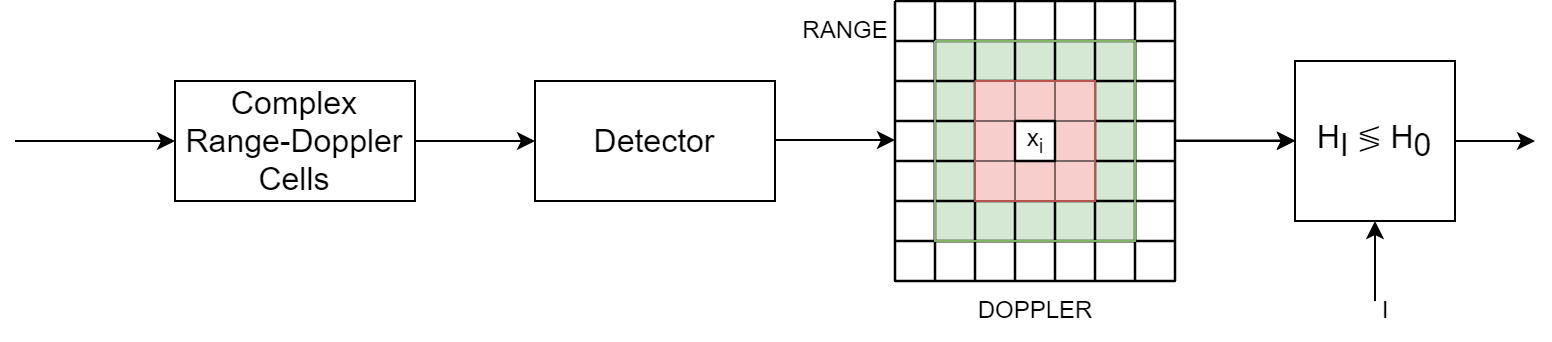
\includegraphics[width=0.9\textwidth]{Images/radar_detect_threshold/cacfar_pipeline.png}
	\caption{CA-CFAR detection processor, guard cells are indicated in red, while reference cells are highlighted in green.}
	\label{fig:cacfar_pipeline}
\end{figure}


% TODO: insert CACFAR scheme from presentation (add guard cells)
% TODO: insert sliding windows

The CA-CFAR threshold is defined by the product of the noise power estimate and a CFAR constant

\begin{align}
	T = \alpha_{\text{CA}} \hat{\sigma_N}^2.
\end{align}

The CFAR constant $\alpha_{\text{CA}}$ is a function of the probability of false alarm $p_{\text{FA}}$ and of the number of contribution cells $N$ and is derived as in chapter 16.5 of \cite{Richards_Scheer_Holm_2010}. The estimated noise power is calculated as in \ref{align: threshold_noise_power} by averaging over the contributing cells

\begin{align}
	\alpha_{\text{CA}} =& N[p_{\text{FA}}^{-1/N} - 1] \\
	\hat{\sigma_N}^2 =& \frac{1}{N}\sum_{n=1}^N z_n.
\end{align}

The number of operations can be reduced by simplifying the normalization by $\frac{1}{N}$ by defining a noise statistics $\hat{g}_{\text{CA}}' = \sum_{n=1}^N z_n$ and by incorporating it in the CFAR constant $\alpha_{\text{CA}}' = p_{\text{FA}}^{-1/N} - 1$.

Computationally CA-CFAR is more demanding than other thresholding techniques, as in its fastest implementation it still requires a 2D convolution to be applied to the periodogram before computing the threshold at each bin.

\subsubsection{Performance of CA-CFAR}

In a heterogeneous environment multiple targets and changes in the interference power degrade CFAR performance. If target returns are present in the reference window, they will bias the threshold and lead to a missed detection. This phenomenon is called \textit{target masking}. Another source of performance degradation is the presence of clutter, where \textit{clutter boundaries} are zones in which there is a sudden change in the statistics of the interfering power.

Performance is also strongly influenced by the design of the reference window. The window should be designed to be as small as possible, in order to reduce the computational load due to the convolution operation and not to include interfering statistics far away from the CUT. The guard interval should be dimensioned according to the point spread function of the target return. An extended target could be counted in the reference window and lead to \textit{self masking}.

\begin{figure}[H]
	\centering
	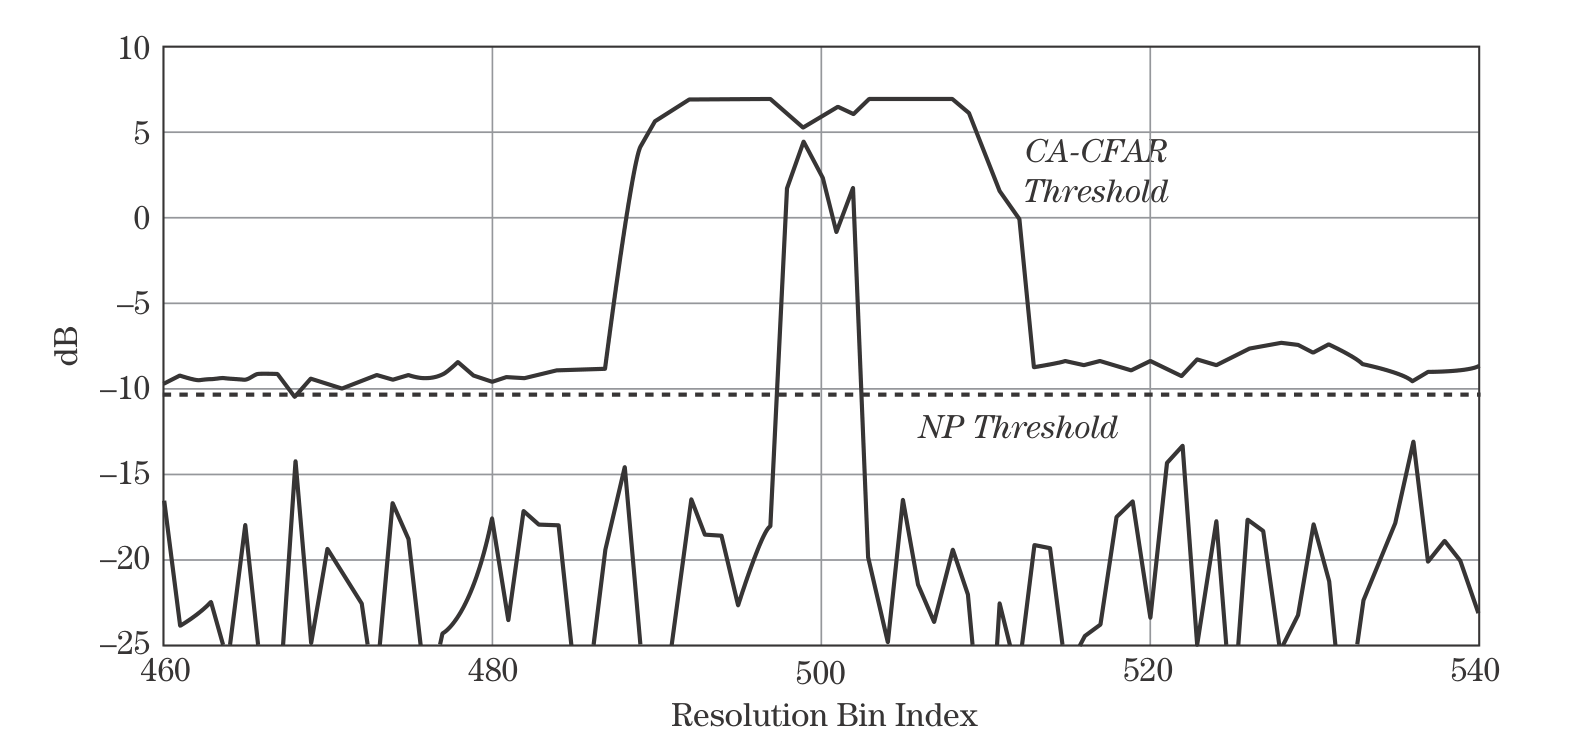
\includegraphics[width=0.7\textwidth]{Images/radar_detect_threshold/self_masking_Richards2010.png}
	\caption{Example of self masking in a 1D radar signal \cite{Richards_Scheer_Holm_2010}}
	\label{fig:self_masking_Richards2010}
\end{figure}


In a NLOS sensing scenario, CA-CFAR suffers from these drawbacks due to the lower SNR of target returns caused by multiple reflections and the presence of strong clutter components close to the zero-doppler bin. Additionally, as NLOS returns propagate over a larger distance their PSF in the periodogram can assume a form similar to clutter. As a result, they do not appear as distinct peaks, but rather are spread across neighbouring bins, which raises the CA-CFAR threshold and leads to missed detections.



\alert{REGENERATE FIGURES, SMALLER, LOWER RANGE, SPEED}
	\begin{figure}[H]
	\centering
	
	\subfloat[Above-threshold bins using CA-CFAR.\label{fig:RadThesh_CA_CFAR_missed_detect}]{%
		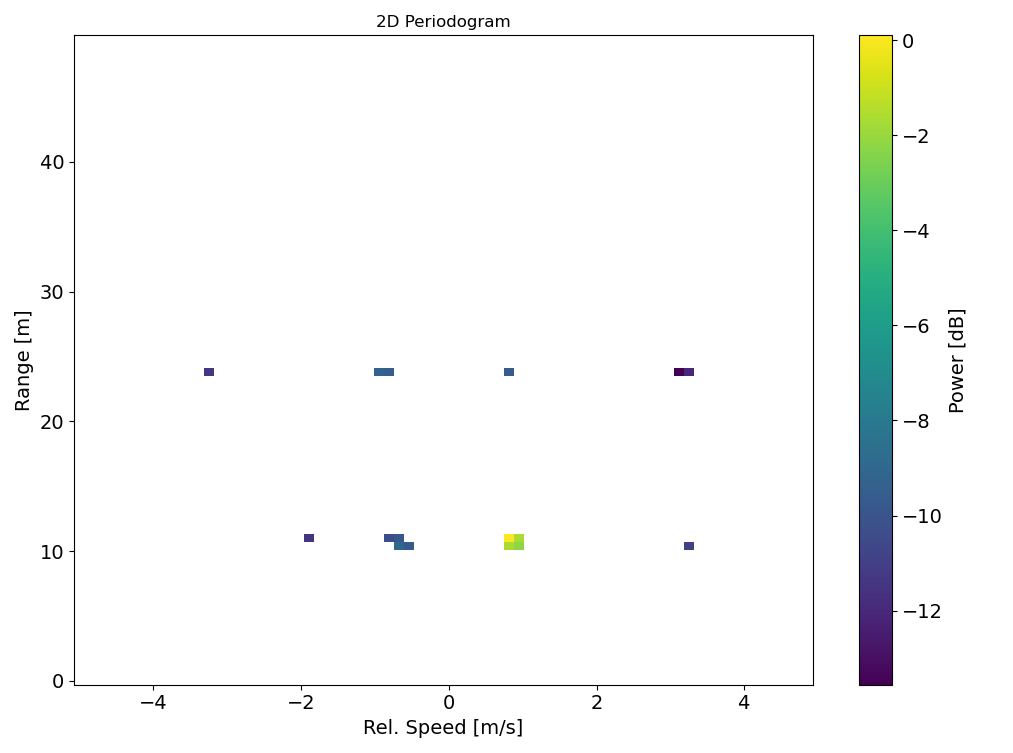
\includegraphics[scale=0.3]{Images/radar_detect_threshold/ca_cfar_no_nlos.png}%
	}\hfill
	\subfloat[Periodogram of the windowing function, FFT over 2048 points.\label{fig:RadThesh_CA_CFAR_missed_detect_PER}]{%
		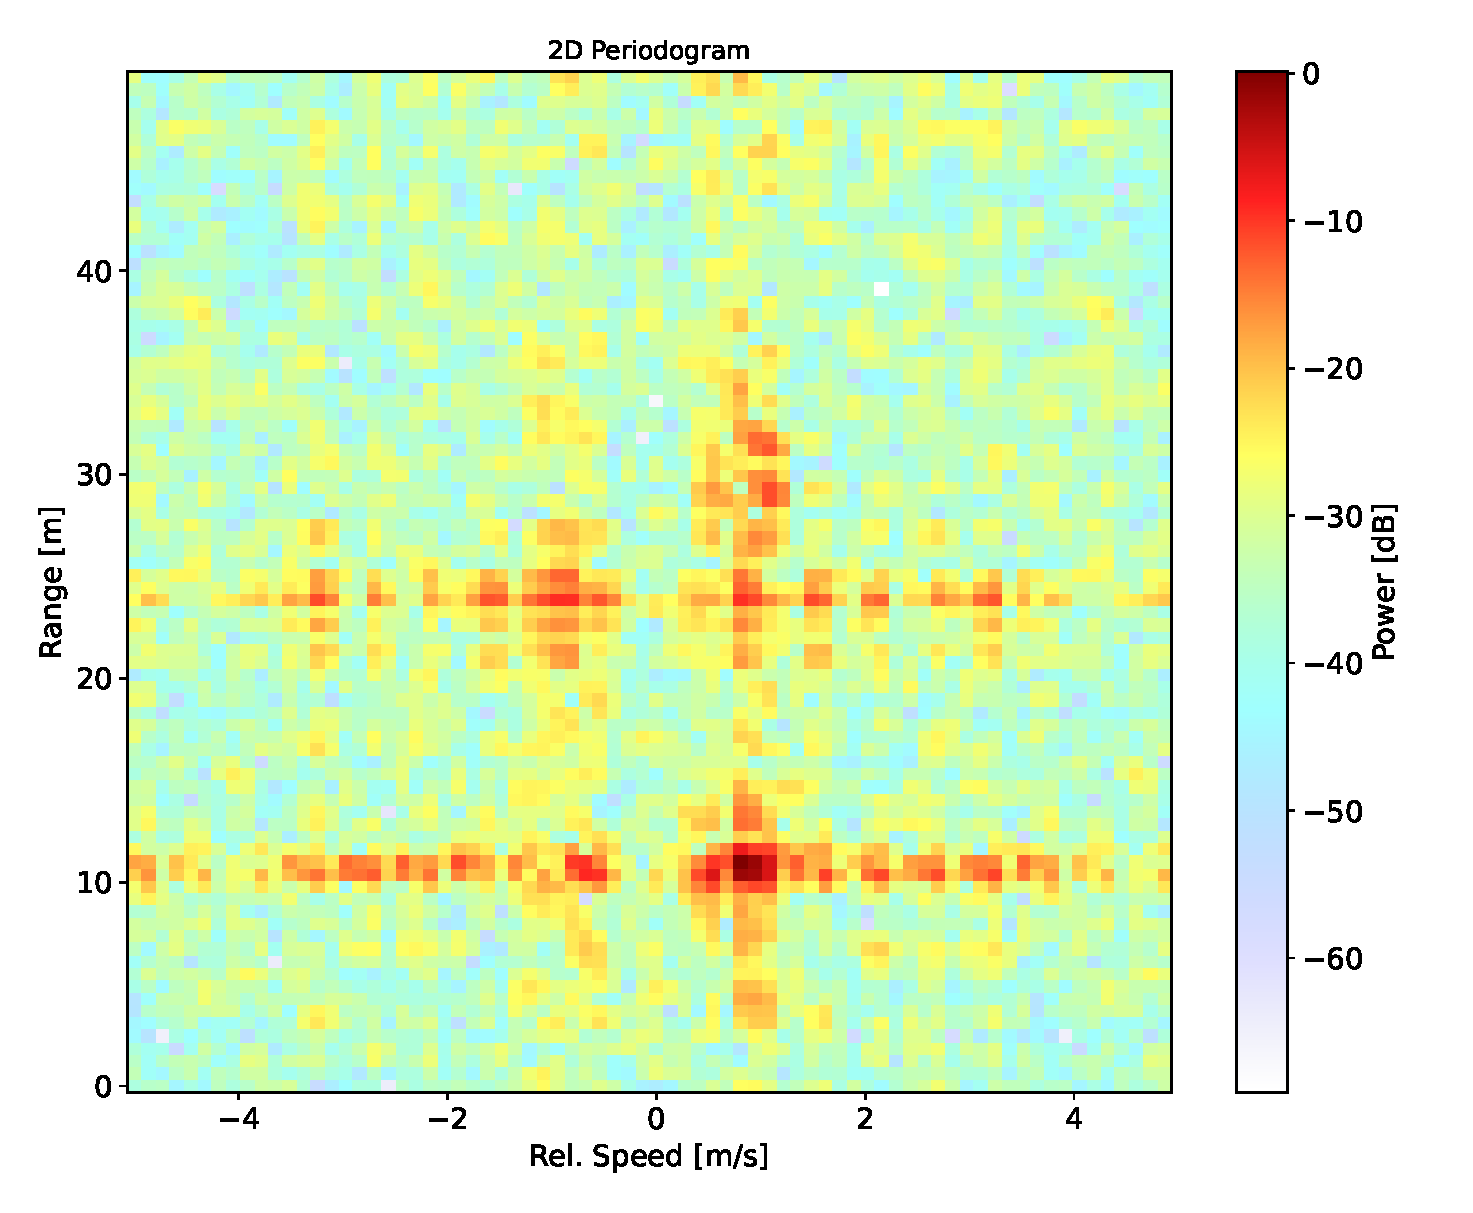
\includegraphics[scale=0.3]{Images/radar_detect_threshold/ca_cfar_no_nlos_PER.eps}%
	}
	
	\caption[]{}
	\label{fig:CA_CFAR_missed_detect}
\end{figure}


\subsection{Robust CA-CFAR}
More complex CA-CFAR algorithms may provide better results under certain heterogeneous conditions, but at the expense of increased computational complexity, higher cost, or lower performance under non-ideal conditions.

Some of the more common variations of the algorithm are the greatest-of CA-CFAR (GOCA-CFAR) and the censored statistics CA-CFAR (CSCA-CFAR), which are designed to suppress clutter-edge false alarms and mutual target masking, respectively.

\paragraph{Greatest-of CA-CFAR:}
the interference power is calculated in the lagging and leading reference windows separately and the largest of the two is selected as the reference statistics. In the OFDM radar signal the leading/lagging definition can be applied only in the doppler dimension, since interference statistics is assumed homogeneous in range.

For the purpose of moving target detection in NLOS clutter-edge false alarms are not a real issue, since bins at zero-doppler are not processed.
 The main problem is given by masking due to the presence of spectral artifacts or clutter.
 
 
\paragraph{Censored-statistics CA-CFAR:}
this algorithm considers the largest $N_c$ samples to be containing returns from interfering targets, and therefore does not consider them when computing the interference statistics. CSCA-CFAR is in general assumed to be capable of removing up to $N_c$ interfering targets.
This algorithm can be also generalised by censoring an arbitary number of samples in order to be adapted to different environments. 

The main limitation posed by this algorithm is the increased computational cost due to the necessary ordering of the interference samples.


\section{Range-adjusted exponential threshold}

In the measurement scenarios it happened that, due to the systems's high range and doppler resolution, target returns presented a point spread function that occupied multiple cells of the periodogram. On the other hand, spectral artifacts due to decimation and/or combining of radio frames kept their original shape in the range/doppler plane. This phenomena is accentuated when windowing the signal before computing the periodogram.

The main consequence is that target returns end up appearing like clutter to the CA-CFAR thresholding algorithm, and no NLOS target falls above threshold.

As proposed in \cite{Wagner_Feger_Stelzer_2017}, a threshold with $1/R^2$ shape can be used to address the problem. This approach is able to identify the target returns, as well as unwanted components. Since this components appear as static in the range/doppler plane, they can be filtered out using a simple Kalman filter. Since their range does not change even though their relative speed is not zero, the filter will update its covariance matrix at each step until a certain threshold is exceeded.





